% TODO fix citation style
% TODO make printbibliography work
% TODO why aquaponics? Why it is so important?

\documentclass[10pt,a4paper]{article}
\usepackage[utf8]{inputenc}
\usepackage[english]{babel}

\usepackage{csquotes}
\usepackage{hyperref}
\usepackage{graphicx}
\usepackage{amsmath}

\usepackage{sty/usecases}
\usepackage{sty/arduinoListing}

\usepackage[
backend=biber,
%style=alphabetic,
%citestyle=authoryear 
]{biblatex}

\usepackage{float}

\floatstyle{plain} % optionally change the style of the new float
\newfloat{Code}{H}{myc}

\addbibresource{jabref.bib}

\title{Armoniacs: Automatized Aquaponics with Arduino}
\author{Guilherme Alcarde Gallo \and Christian Esteve Rothenberg 
%\and Edmundo Roberto Mauro Madeira
}

% define \req command to label requirements in description environment
\makeatletter
\newcommand{\req}[1]{
  \def\@currentlabel{R#1}\label{req#1}
  \textbf{R#1}
}
\makeatother

\begin{document}

\maketitle

\newpage

\tableofcontents

\newpage

\section{Introduction}
\label{sec:introduction}
\subsection{Motivation}
Basically,
the automation purpose is to save labor and add more security,
precision and velocity to tasks that formerly were made by humans or other animals.

If someone wonder about the reason for automating tasks,
this person needs to pay attention about living in modern civilizations.
When one walks on the sidewalk,
one can see vehicles parked on the road,
these are automated objects,
because saves the labor of walking to distant places --
or making animals to walk for us --
via the electronic management of several components,
such as acceleration,
fuel measurement,
injection,
breaking with ABS technology etc.
But not only cars are automated.
The microwave,
airplanes and elevators are automated objects which are used frequently.

Generally, 
an automation project is composed by a microcontroller, 
electronic devices and a variable number of sensors.
The former is the main component,
which is responsible to manage the system by reading the input from the latter,
and then process what to do,
so it can send signals to electronic devices to accomplish the system's goal.
This processing is made with programming.
A programmer can install the code inside the microcontroller,
which will execute the program when turned on.
So it is presupposed that the programmer will align the program with the system's intention.

\subsubsection{Context}
When someone builds an Aquaponics system,
one needs to manage it everyday,
since there is a plenty of work to do for maintaining the system work,
due the dependency of living beings on the system.
So it is a time wasting management,
with lots of repetitive tasks,
which one can be understood as periodic events.
Other tasks needs precision,
such as water leveling and pH balancing,
that feature can be achieved with automation.

Some of these tasks can be reliably automated,
together with others that involves problems that may occur during the system's growth.
For example, the fish feeding is a periodic event,
but the water's pH control is not a periodic event,
instead it is classified as an adverse event.

Basically this work is trying to decrease human intervention in an Aquaponics system via automatic management of adverse and periodic events,
in order to reduce the time wasted to take care of the system, 
as well as to make the management more reliable.

The figure \ref{fig:aquaponicsExample} demonstrate an example of a functional Indoor Growing System applying Aquaponics.

\paragraph{Reasons to build an Aquaponics system}

A great amount of the published projects has a commercial goal:
to make an efficient and small-sized system that can afford to produce organic products in a large scale.

On other hand,
in the \cite{GoddekDelaideMankasinghEtAl2015} there is an effort to address the sustainability aspect of the Aquaponics.
This aspect stands for making a low and efficient nutrient input into the system and making a minimal environment footprint.

\paragraph{Differences between Hidroponics and Aquaponics}

The Hidroponics is a system that uses a nutritive water to feed the plants.
It is a inorganic system, 
where the addition of inorganic nutrients is needed and the main live component is the plant.
On the other hand, the Aquaponics is a partly-organic system cite,
where the fish is added to the system,
and its waste,
the ammonia,
serves as a nutrient to the plants.

The great advantage of the Hidroponics over the Aquaponics is that the last may have some issues with human diseases,
like the presence of snails with parasites in the fish tank or some water-borne disease. \cite{wilson2005greenhouse}.

\begin{figure}[h]
    \centering
    \includegraphics[width=.5\textwidth]{img/aquaponics.png}
    \caption{An example of a built Aquaponics system. The plant medium is above and at the right of the electronic pump. At the bottom is the fish tank. \cite{goldstein2013indoor}}
    \label{fig:aquaponicsExample}
\end{figure}


\subsection{Challenges}

\subsubsection{Without automation}
To build an Aquaponics system,
one needs to be precise and cautious when one makes the design of the project,
since there are lots of requirements that need to be respected in order to make the Aquaponics work.
The most important requirements are strongly connected with equilibrium,
because we are dealing with a biological system.
For example,
the proportion between the fish tank and the plant's grow bed tank are vital to optimize.
If one gets the wrong proportion,
the system won't work,
both the fish and the plants will die precociously \cite{Leatherbury2014}.

Another problem is to distribute the byproducts of each medium to another one,
the main byproduct of the fish tank is ammonia,
if the concentration of the latter increases,
the fish will die by high toxicity,
hence this ammonia has to be delivered to the bacteria,
who will digest this substance via the nitrogen cycle,
producing nitrate.

As the final product are comestibles,
there is another concern: food toxicity.
One cannot use components made with materials that can cause water contamination,
because the fish and the plant will be contaminated as well.
So there is the need to use non-toxic elements in the system.
Besides there is also a high concern with the water source,
the water cannot be infected with pathogens that causes diseases,
like amoeba.

Lots of research have been done about the biological aspect of the Aquaponics.
In \cite{GoddekDelaideMankasinghEtAl2015},
the authors show high complexity problems involving mechanisms to achieve pH equilibrium for optimizing the quality of life for the fish,
plants and nitro-bacteria,
since each living component of the system lives well in a certain pH-Range.
So there is a challenge to separate the pH level by region.
Despite of the requirement \ref{req2} treats the pH level of all mediums monolithically,
the dedicated controlling of each medium's pH level is not treated in this work,
for the sake of simplicity.

\subsubsection{With automation}
In order to automate an Aquaponics system,
one must take care with microelectronic components,
they have to be protected from water and humidity.

Second,
there is the need to use relays to add high current-drain devices,
like the submersible water pump,
which is essential to the system.
If this advise is ignored,
the microcontroller will be damaged.


\subsection{Project Objectives and Scope}
% Problem characterization and goals
\label{objectives}
Design the proof of concept of a system that is capable to automatically control and optimize the water cycle and its quality of an Aquaponics system via microcontroller.

% Macro and Micro
% What was implemented what wasn't.

What is in the scope of this proof of concept:
\begin{itemize}
    \item Automatized Water Cycling for exchange water between tanks
    \item Water pH Level Automatic Control
\end{itemize}

What is out of scope:
\begin{itemize}
    \item Automatic Fish Feeding
    \item Aquaponics structural design which doesn't regard automation,
        such as: tanks, pipes etc
    \item Root Cloging prevention
\end{itemize}


\section{Theoretical Background and Related Work}
\label{fundamentals}
\subsection{Background}
An extensive research has been made aiming at some basic Aquaponics knowledge and previous Aquaponics automation projects.
The idea for creating a water cycle has came from \cite{simpleArduinoAquaponics},
where a simple project is proposed and an Arduino only automates this very feature of the system.
But the system design of the former project with 3 tanks and 1 second water cycle will not be applied,
the \cite{Kretzinger2015} uses a simpler approach with only 2 tanks and a periodic water cycle,
with the difference that the period is much longer.

There are some projects that uses multiples microcontrollers,
like \cite{GarethColeman2014},
which uses an Arduino Mega with Raspberry PI.
To make the things simpler,
this project focuses on using only one microcontroller.

\subsection{Technologies}
\subsection{Related work}
\subsection{Conclusion}


\section{System Proposal}
\label{proposal}
% V-model
\subsection{Approach}
This work has been implemented with an adaptation of V-model development process
\footnote{Described in detail here: \cite{mathur2010advancements}}.
The original version of this process is known as a variation of the waterfall process,
with several phases that resembles the latter,
but the their displacement is slightly modified,
emphasising on the coding phase.

An appealing feature of the V-model is that every phase,
before the coding one,
has a 1:1 strong relationship with the phases that occurs after the coding,
as seen in figure \ref{fig:v-model},
reinforcing the mapping of the theoretical part of the project with the practical one.
Moreover,
in comparison with Agile models,
there is much more documentation in a project using V-model,
and this feature is crucial for this work.

\begin{figure}[h]
    \centering
    \includegraphics[width=.7\textwidth]{diagrams/traditional_V-Model.jpg}
    \caption{A V-model flow diagram. \cite{vmodelCMU}}
    \label{fig:v-model}
\end{figure}

The adaptation made in this project was to divide the V-model into iterations separated by the use cases.
That is,
for every use case,
there are the execution of every phase of V-model,
as if the product would have only one use case.

After some research about the flaws of V-model,
a variation of the V-model has been found and it shares the fundamental difference between this work's approach and V-model:
the Dual V-model \cite{clark2009system}.
The shared idea is: divide and conquer V-model, 
by making subsystems that follows V-model,
so,
when these subsystems are finished,
they can be integrated to create the final product.

% \subsubsection{How it works}

% \subsubsection{Mapping V-model to this work}
\begin{description}
    \item[$\bullet$ Requirements Analysis] Sections \ref{sec:useCases} and \ref{sec:requirements}
    \item[$\bullet$ Specification / System Design] Section \ref{sec:design}
    \item[$\bullet$ Architectural Design / System Architecture] Section  \ref{sec:architecture}
    \item[$\bullet$ Detail Design / Module Design] Section \ref{implementation}
    \item[$\bullet$ Unit Testing] Section \ref{sec:video}
    \item[$\bullet$ Integration Testing] Section \ref{sec:video}
    \item[$\bullet$ System Testing] Section \ref{sec:video}
    \item[$\bullet$ User Acceptance Testing] Not used, because we are building a proof of concept.
\end{description}


In order to demonstrate the proof of concept without any physical building,
there is a video with a Graphical User Interface in the section \ref{sec:video},
which the user can simulate how the system responds to the undesired pH values in the tank.
This video is made based on the IP Capture library for Processing \cite{ipcapture_2016},
that makes feasible to render life video from a IP camera,
hence it is possible to watch what happens with the Arduino in real-time when one changes a sensor value.

\subsection{Use Cases}
\label{sec:useCases}
\input{useCases/waterCycleControl}
\newpage
%Sometimes it is a good idea to put domain objects in \texttt{}
%The template and the descriptions are based on the book Applying UML and Patterns: 
%An Introduction to Object-Oriented Analysis and Design and Iterative Development
%(3rd Edition) by Craig Larman.
\begin{usecase}

    \addlongtitle{Keep water tank's}{pH level in 6-7 range}{\quad Details} 

%Scope: the system under design
%\addfield{Scope:}{System-wide}

%Level: "user-goal" or "subfunction"
%\addfield{Level:}{User-goal}

%Primary Actor: Calls on the system to deliver its services.
\additemizedfield{Actors:}
{
\item Microcontroller
\item Peristaltic Water Pumps 
\item pH Sensors
}

%Stakeholders and Interests: Who cares about this use case and what do they want?
%\additemizedfield{Stakeholders and Interests:}{
	%\item Stakeholder 1 name: his interests
	%\item Stakeholder 2 name: his interests
%}

%Preconditions: What must be true on start and worth telling the reader?
%\addfield{Preconditions:}{}
%when multiple
\additemizedfield{Preconditions:}{
    \item The Microcontroller, pH sensors and the peristaltic pumps must be installed in the system
    \item A proper relay must be installed in the system
         OR a power transistor to supply 12V DC
    \item The external power supply and the water pump must be compatible
} 

%Postconditions: What must be true on successful completion and worth telling the reader
\addfield{Postconditions:}
{
    The water tank's pH level is between 6 and 7.
}
%when multiple
%\additemizedfield{Preconditions:}{}

%Main Success Scenario: A typical, unconditional happy path scenario of success.
\addscenario{Main Success Scenario:}{
	\item The Microcontroller checks the pH sensor.
    \item The pH output is between 6 and 7.
	%\item The Microcontroller executes a run cycle of 25\% in the PWM in a 1 hour period.
}

%Extensions: Alternate scenarios of success or failure.
\addscenario{Extensions:}{
	\item[2.a] Lower pH values in output:
		\begin{enumerate}
            \item[1.] The circuit sends this signal to start the high pH relay.
            \item[2.] The relay distributes the needed current to the high pH's peristaltic pump.
            \item[3.] High pH water is blended with the water tank's, until the latter gets into the normal pH range.
            \item[4.] The circuit sends this signal to stop the high pH relay.
		%\item[2.] User returns to step 1
		\end{enumerate}
	\item[2.a] Higher pH values in output:
		\begin{enumerate}
            \item[1.] The circuit sends this signal to start the low pH relay.
            \item[2.] The relay distributes the needed current to the low pH's peristaltic pump.
            \item[3.] High pH water is blended with the water tank's, until the latter gets into the normal pH range.
            \item[4.] The circuit sends this signal to stop the low pH relay.
		%\item[2.] User returns to step 1
		\end{enumerate}
	%\item[5.a] Invalid subsriber data:
		%\begin{enumerate}
		%\item[1.] System shows failure message
		%\item[2.] User returns to step 2 and corrects the errors
		%\end{enumerate}
}

%Special Requirements: Related non-functional requirements.
\additemizedfield{Special Requirements:}{
	%\item R1: Operation Time Limit requirement
	\item \ref{req2}
}

% TODO: COOL Technology and Data Variations List: Varying I/O methods and data formats.
%\addscenario{Technology and Data Variations List:}{
	%\item[1a.] Alternative first action with other technology
%}

%Frequency of Occurrence: Influences investigation, testing and timing of implementation.
%\addfield{Frequency of Occurrence:}{}

%Miscellaneous: Such as open issues/questions
%\addfield{Open Issues:}{}

\end{usecase}


\subsubsection{Summary table}

\begin{table}[h]
\centering
\caption{Requirements table}
\label{tab:requirementsTable}
\begin{tabular}{|c|c|c|}
\hline
\textbf{Use Case}    & \textbf{Requirement} & \textbf{References} \\ \hline
Optimize Water Cycle & \ref{req1}           &                 \\ \hline
Keep pH Level optimum & \ref{req2}           &  \cite{tables} \\ \hline
\end{tabular}
\end{table}

\subsection{Requirements}
\label{sec:requirements}

\begin{description}

\item [\req{1}]
Optimize the water cycle period between fish tank and plants medium.

\item [\req{2}]
Keep the pH Level around the 6-7 range.

\end{description}

\subsection{System Design}
\label{sec:design}

The figure \ref{fig:highLevelSystemDesign} shows a high level diagram to demonstrate how the automation can be implemented in the Aquaponics.
Each node has an input and output,
indicated by an incoming and outgoing arrows, respectfully.

The components are from the original Aquaponics system,
which are surveyed by the sensors.
The latter captures dedicated data from the medium,
like temperature or water level and emits an electronic signal to the microcontroller.

The latter is the main responsible for the automation,
it is where the logic is stored,
so the input signal are interpreted by the installed program and another electronic signal is sent to the components,
this signal could be directed or indirect,
the former is when the output current is enough to the target component to work,
otherwise the latter is used via a relay,
that is connected with an external power supply,
and behaves as an signal amplifier.

\begin{figure}[h]
    \centering
    \includegraphics[width=.7\linewidth]{diagrams/systemDesign}
    \caption{A simple diagram to represent a high level design of this project}
    \label{fig:highLevelSystemDesign}
\end{figure}

\subsection{System Architecture}
\label{sec:architecture}

Figure \ref{sec:architecture} illustrates the low-level design.
Based on the figure \ref{fig:highLevelSystemDesign},
the figure \ref{fig:waterCycleDiagram} depicts a model to automatize the water cycle control from the requirement \ref{req1}.
Now one can see where to connect each terminal and every important component is presented.

\begin{figure}[h]
    \centering
    \includegraphics[width=.6\linewidth]{diagrams/architecture_bb}
    \caption{This diagram shows how the microcontroller interacts with the water pump}
    \label{fig:waterCycleDiagram}
\end{figure}

Each wire color has a meaning.
Blue represents the ground voltage,
red is high voltage
and yellow is low voltage.
The submersible water pump is located inside the fish tank and normally is turned off.
When the periodic signal comes from the microcontroller's digital output,
it is amplified by the relay switching,
which in turn makes the power supply to deliver high voltage to the water pump,
the latter works until the relay is switched again by the microcontroller's signal downtime.

\subsection{Project Decisions}
There are a lot of authors \cite{GoddekDelaideMankasinghEtAl2015} \cite{clark2009system} \cite{Leatherbury2014} that have had experience with Aquaponics automation.
Most of them chooses Arduino or Raspberry Pi as the main microcontroller.

Two great reasons for the Arduino's usage are:
This work's author already has an Arduino UNO,
but not a Raspberry PI.
Besides the main reference of this work,
the \cite{Kretzinger2015},
whose author has many years of experience with Aquaponics and its automation and he uses the Arduino as microcontroller.

The chosen components have been based in the references.


\section{Implementation}
\label{implementation}
\subsection{Periodic Water Cycling Code}

%\minisec{Sketch 1: A flashing LED on a protoboard}

\begin{lstlisting}[style=Arduino, caption=Water Cycle First Code, label=lst:water1]
 /*  Emits a periodic signal one quarter per hour */

// Which pin is connected with the water pump?
const int waterPumpPIN = 4;

// Time intervals
// 15 min = 60e3 ms * 15 = 9e5 ms
const int fifteenMin = 900000;
const int fourtyFiveMin = 2700000;

void setup(){
  // Sets the waterPumpPIN as the output of the periodic signal
  pinMode(waterPumpPIN, OUTPUT);
}

void loop(){
  digitalWrite(waterPumpPIN, HIGH); // sets the signal to logical 1 ON
  delay(fifteenMin // stay on high voltage for 15 minutes
  digitalWrite(waterPumpPIN, LOW); // sets the signal to logical 0 OFF
  delay(fourtyFiveMin); // stay on low voltage for 45 minutes
}
\end{lstlisting}

% Make a second code based on https://www.arduino.cc/en/Tutorial/BlinkWithoutDelay
\subsubsection{Reviewed Code}
A program that uses delay in the main loop to make timed actions is error-prone,
since the delay will be belated by the overhead of other operations located inside the main loop.
Moreover the Arduino will not detect any interruption during a delay,
so we need to use delays only when it is really necessary.

To make a better code and to improve the scalability of the automation for more use cases that needs to be precisely timed,
one needs to review the code to find another way to do periodic actions.
We used \cite{arduinoDelay} as a reference to remove the delay-based code from water cycling's code \ref{lst:water1}.

\begin{lstlisting}[style=Arduino, caption=Water Cycle Code without Delays]
 /*  Emits a periodic signal one quarter per hour
     without using delay */

// Which pin is connected with the water pump?
const int waterPumpPIN = 4;

// State of the signal
int waterPumpState = LOW;

// Using unsigned variable to support more data
unsigned long previousMillis = 0;

// Time intervals
// 15 min = 60e3 ms * 15 = 9e6 ms
const int fifteenMin = 9000000;
const int fourtyFiveMin = 27000000;

void setup(){
  // Sets the waterPumpPIN as the output of the periodic signal
  pinMode(waterPumpPIN, OUTPUT);
}

void loop(){
  digitalWrite(waterPumpPIN, HIGH); // sets the signal to logical 1 ON
  delay(fifteenMin // stay on high voltage for 15 minutes
  digitalWrite(waterPumpPIN, LOW); // sets the signal to logical 0 OFF
  delay(fourtyFiveMin); // stay on low voltage for 45 minutes
}
\end{lstlisting}

Note that we are storing the timestamps in a 32-bit variable,
so the overflow will occur in almost 50 days,
because the limit is $ ( 2^{32} -1 ) $ ms.
But there is a fancy property with this overflow that soothes this worry:
the subtraction of two timestamps will remain correct even if there is a overflow in those numbers,
given that the variable is unsigned.
$ limit = FFFF FFFF $
$ limit - 3 seconds = FFFF FFFB $
$ limit + 1 = 0 $
$ 10 seconds = A = limit + B $
$ 0000 000A - FFFF FFFB = 0000 000E = 14 seconds $


% Evaluation
% Related with the requirements:
% Test 1: R1: pH Control: change constant's value and verify control work
\section{Results and Evaluation}
\label{evaluation}
% Evaluation
% Related with the requirements:
% Test 1: R1: pH Control: change constant's value and verify control work

\subsection{The Circuit Setup}

% \begin{figure}[h]
%     \centering
%     \includegraphics[width=.7\textwidth]{img/photo1.png}
%     \caption{A photo of the Water Cycle Control Circuit}
%     \label{fig:photo}
% \end{figure}

\subsection{A Graphical User Interface}

For the sake of making the unit tests to be shown in a written report,
a simple Graphical User Interface (GUI) has been implemented using Processing.
Processing is a simple programing language which is integrated with OpenGL,
Java and Serial communication.
So it is a reliable choice to display and transmit Serial data from/to Arduino within the computer screen.
But,
instead of being a monitoring-only GUI,
the Processing provides built-in functions to make mouse interactions easily,
hence the tests could be made faster.

\begin{figure}[h]
    \centering
    \includegraphics[width=.7\textwidth]{img/gui1.png}
    \caption{An initial version of the GUI}
    \label{fig:gui}
\end{figure}

\begin{figure}[h]
    \centering
    \includegraphics[width=.7\textwidth]{img/gui2.png}
    \caption{Using the G4P plugin for processing to make GUIs}
    \label{fig:g4p}
\end{figure}


\newpage
\section{Conclusion}
\label{conclusion}
% Which were the difficulties?
% Is there any POC?
% What is the contribution of this work?

As the author of this work did not have the enough experience with microelectronics,
because he had been doing the software-biased modality of his degree,
he had some difficulties relating the schematics designs,
how to use relays and other advanced components.


% \section{State of Art}
% \label{sec:state_of_art}

% There are some automated aquaponics projects available on the Internet,
but most of them doesn't have a reasonable good documentation.
So it has been needed to grab parts of information among every material found on Internet.
One of the best sources found was from a hackaday's post from \cite{gareth_coleman_aquapionics_2016},
which describes with decent detail how they achieved the construction of their Arduino-powered aquaponics system.

Lots of research have been done about aquaponics.
In \cite{goddek2015challenges}, the authors show high complexity problems involving mechanisms to achieve pH equilibrium for optimizing the quality of life for the fish, plants and nitro-bacterias.
Since each living component of the system lives well in a certain pH-Range.
So there is a challenge to separate the pH level by region.

\subsection{Why people are interested in Aquaponics?}

A great amount of the published projects has a commercial goal:
to make an efficient and small-sized system that can afford to produce organic products in a large scale.

On other hand,
in the \cite{goddek2015challenges} there is a try to address the sustainability aspect of the aquaponics
This aspect stands for making a low and efficient nutrient input into the system and making a minimal environment footprint.


% \section{Required Components}
% \label{sec:required_components}

% \begin{description}
    \item[Arduino UNO] \hfill \\
        Some project authors recommends the Arduino MEGA because of its extra GPIO pins.
        But we only have the UNO version by now.
    \item[DC Motor] \hfill \\
        A simple DC Motor can be enough for this project.
        It could be used to feed the fish periodically.

        There is a simple mechanism inspired by the video \cite{judoisonattack2012},
        where the fish food is wrapped in a pot and rotated down just for a arbitrary short time,
        and then rotated back up.
        It can be controlled by sending electrical current timed by the Arduino.
    \item[Waterproof Temperature Sensor] \hfill \\
        This item is necessary for monitoring whether the fish's ambient is favorable for the fish.
    \item[Water Level Sensor] \hfill \\
    \item[Water Pump] \hfill \\
        Needed to give potential energy to the water flow,
        being fundamental to the water's cycle.
    \item[pH and ORP probe] \hfill \\
        pH levelling is an essential feature of the system.
        The fish, the nitro-bacterias and the plants needs to live in a specific pH-range ambient.
        With the probe,
        when the ambient is suffering with a pH decreasing,
        the system could automatically drop some amount of CaCO3 into the water to rise the pH from the fish tank,
        for example.
    \item[Relay Board] \hfill \\
        Some items,
        like the Water Pump,
        draws too much current if compared with Arduino's capacity.
        So one needs to use relays to connected another power source with the Arduino's output signals.
\end{description}


% \section{Proof of Concept}
% \label{sec:proof_of_concept}

%% The initial idea is to make a emulated system as a proof of concept of the aquaponics system automatization.
There are some softwares that can help the project to achieve its goals.

List of softwares:
\begin{itemize}
\item{Autdesk 123D}
\item{Node-RED}
\item{Fritzing}
\end{itemize}


\subsection{Guidelines}
A Do It Yourself (DIY) online magazine called Makezine,
has an article \cite{make_mag_Arquaduinic} that presents some rules to make a durable aquaponics.

Some common problems presented by this article:
\begin{itemize}
    \item Some plant roots clogs the water outputs
\end{itemize}<++>


\newpage
\nocite{useCaseStyle}
\printbibliography

\end{document}
